\documentclass[utf8]{beamer}

\usepackage[T1]{fontenc}
\usepackage[brazil]{babel}
\usepackage{inconsolata}
\usepackage{minted}
\usepackage{tabu}
\usepackage[absolute, overlay]{textpos}
\usepackage{graphicx}
\usepackage{changepage} % adjustwidth environment
\usepackage{qrcode}
\usepackage{tikz}

\definecolor{codebgcolor}{HTML}{FFFFFF}
\definecolor{coderulecolor}{HTML}{5F7FFF}
\definecolor{outerbgcolor}{HTML}{FCFCF0}

\setminted{autogobble,
           breaklines, breakanywhere,
           breaksymbolindentleft=0pt, breaksymbolindentright=0pt,
           breaksymbolsepleft=3pt, breaksymbolsepright=3pt,
           breaksymbolright=...,
           bgcolor=codebgcolor, style=paraiso-light,
           fontsize=\fontsize{10pt}{10pt},
           frame=lines, rulecolor=coderulecolor, framerule=.7pt}
\setmintedinline{bgcolor={}}

\mode<presentation>
\usetheme{Warsaw}
\setbeamercolor{structure}{fg=purple!20!black}
\setbeamercolor{background canvas}{bg=outerbgcolor}
\beamertemplatenavigationsymbolsempty

\setbeamertemplate{footline}{\leavevmode\hbox{%
  \begin{beamercolorbox}[wd=.35\paperwidth, ht=2.25ex, dp=1ex, center]
                        {author in head/foot}
    \usebeamerfont{author in head/foot}
      Danilo J. S. Bellini \hfill \texttt{@danilobellini}
  \end{beamercolorbox}%
  \begin{beamercolorbox}[wd=.65\paperwidth, ht=2.25ex, dp=1ex, center]
                        {title in head/foot}
    \usebeamerfont{title in head/foot}
      \insertshorttitle \hfill
      SSI-IX @ EACH-USP -- SP \hfill
      \insertshortdate \hfill
      \insertframenumber\,/\,\inserttotalframenumber
  \end{beamercolorbox}%
}}

\setbeamertemplate{background}{%
  \tikz[overlay,remember picture]%
    \node[opacity=0.05]at (current page.center){%
      
\includegraphics[height=.7 \paperheight]{logo_ssi.png}%
    };%
}


\title{Introdução à Criptografia}
\subtitle{Fundamentos e aplicação prática}
\author{Danilo J. S. Bellini \\ \texttt{@danilobellini}}
\date{2019-08-12}

\setlength{\TPHorizModule}{\paperheight}
\setlength{\TPVertModule}{\paperheight}

\renewcommand{\thefootnote}{[\arabic{footnote}]}

\newcommand{\includesvg}[2]{%
  \ifnum\pdfstrcmp{\pdffilemoddate{#2.svg}}%
                  {\pdffilemoddate{#2.pdf}}>0%
    {\immediate\write18%
     {inkscape -z -D --file=#2.svg --export-pdf=#2.pdf --export-latex}%
    }%
  \fi%
  \centering%
  \resizebox{#1}{!}{%
    \input{#2.pdf_tex}%
  }%
}

\newcommand{\uppera}[0]{\textsuperscript{\b{a}}~}
\newcommand{\repo}[0]{https://github.com/danilobellini/slides-latex}

\newcommand{\secAddressOne}[0]{%
  https://www.quora.com/What-is-the-difference-between-the%
                                   -words-safe-and-secure%
}
\newcommand{\secAddressTwo}[0]{%
  http://www.iot.ntnu.no/users/albrecht/rapporter/%
                                  notat\%20safety\%20v\%20security.pdf%
}
\newcommand{\challengeOne}[0]{ETKRVQITCHKC}
\newcommand{\challengeOneKey}[0]{C}
\newcommand{\challengeTwo}[0]{ERCYEQWHVA}
\newcommand{\challengeTwoKey}[0]{EACH}
\newcommand{\challengeThree}[0]{WSBKSQBS}
\newcommand{\challengeThreeKey}[0]{USP}
\newcommand{\challengeFour}[0]{$p=41$, $g=2$, $a=5$ e $B=32$}
\newcommand{\challengeFive}[0]{1234-527\_}

\begin{document}


\begin{frame} \vspace{2cm}
  \titlepage
  \center
    {\huge 9\uppera Semana de Sistemas de Informação}
  \begin{textblock}{0}(.05, .05)%
    
\includegraphics[height=50pt]{logoeach2.png}%
  \end{textblock}
  \begin{textblock}{0}(.8, .05)%
    
\includegraphics[height=50pt]{IXSSI-768x294.jpg}%
  \end{textblock}
  \begin{textblock}{.4}(.07, .53)%
    
\includegraphics[height=50pt]{Logo_EACH-USP.png}

    Escola de Artes, Ciências e Humanidades%
  \end{textblock}
  \begin{textblock}{.3}(.93, .6)
    
\includegraphics[height=20pt]{usp.png}

    Universidade de São Paulo%
  \end{textblock}
\end{frame}


\begin{frame}{O que é segurança?}
  Estar livre de perigos? Minimizar riscos?
  \vfill
  Em inglês há duas palavras: safety VS security\footnote{
    Para definições mais completas dessas palavras, veja
    \url{\secAddressOne} e \url{\secAddressTwo}
    (\emph{links} nos respectivos \emph{QR codes} acima).
  }
  \begin{itemize}
    \item \emph{Safe} refere-se à proteção
          sobre acontecimentos indesejáveis do acaso.
          No limite, pode ser usado para indicar que algo é autêntico,
          não uma fraude;
    \item \emph{Secure} refere-se à proteção
          contra acontecimentos intencionais.
          Em geral, é aqui que se encaixa a segurança da informação.
  \end{itemize}
  \vfill
  Aspectos da segurança da informação:
  \begin{itemize}
    \item Confidencialidade / Privacidade
    \item Integridade
    \item Disponibilidade
  \end{itemize}
  \begin{textblock}{0}(.8, .55)%
    \qrcode{\secAddressOne}~\hspace{.5cm}~\qrcode{\secAddressTwo}%
  \end{textblock}
\end{frame}


\begin{frame}{Criptografia}
  Criptografia é a \emph{prática} e o \emph{estudo}
  das técnicas de armazenamento e comunicação de informação
  na presença de terceiros/adversários.
  Aspectos da segurança da informação (\emph{security}):
  \vfill
  \begin{itemize}
    \item
    Integridade:
    \textbf{Assinatura} (\emph{Sign})
    \item
    Confidencialidade / Privacidade: \\
    \textbf{Encriptação/decriptação} (\emph{Encrypt/Decrypt})
  \end{itemize}
  \vfill
  Classificamos os algoritmos de acordo com o número de chaves:
  \vfill
  \begin{itemize}
    \item Criptografia de chave simétrica \\
          (chave única, de conhecimento exclusivo das partes)
    \item Criptografia de chave pública \\
          (chave pública e chave privada formando um par)
    \item Funções de \emph{hash} (sem chave)
  \end{itemize}
  \begin{textblock}{0}(1, .01)%
    \includesvg{70pt}{Crypto_key}%
  \end{textblock}
\end{frame}


\begin{frame}{Chave simétrica: Cifras de César}
  \vspace{-.3cm}
  \begin{center}
    \resizebox{.8 \textwidth}{!}{%
      \begin{tabular}{rl}
                Chave: & \texttt{C} \hfill
                         \emph{\tiny(Desloca 2 no alfabeto,
                                     A \textrightarrow C)} \\
        Chave efetiva: & \texttt{CC CCCCC CC CCCCCCCC} \\ \hline
             Mensagem: & \texttt{EU GOSTO DE LIMONADA} \\
        Texto cifrado: & \texttt{GW IQUVQ FG NKOQPCFC} \\
      \end{tabular}%
    }
  \end{center}
  \vfill
  A cifra de César transforma cada caractere da mensagem
  usando uma tabela como esta:
  \vspace{.3cm}
  \vfill
  \resizebox{\textwidth}{!}{%
    \begin{tabular}{c|c|c|c|c|c}
      \texttt{A} \textrightarrow \texttt{C} &
      \texttt{B} \textrightarrow \texttt{D} &
      \texttt{C} \textrightarrow \texttt{E} &
      \texttt{D} \textrightarrow \texttt{F} &
      \texttt{E} \textrightarrow \texttt{G} &
      \texttt{F} \textrightarrow \texttt{H} \\
      \texttt{G} \textrightarrow \texttt{I} &
      \texttt{H} \textrightarrow \texttt{J} &
      \texttt{I} \textrightarrow \texttt{K} &
      \texttt{J} \textrightarrow \texttt{L} &
      \texttt{K} \textrightarrow \texttt{M} &
      \texttt{L} \textrightarrow \texttt{N} \\
      \texttt{M} \textrightarrow \texttt{O} &
      \texttt{N} \textrightarrow \texttt{P} &
      \texttt{O} \textrightarrow \texttt{Q} &
      \texttt{P} \textrightarrow \texttt{R} &
      \texttt{Q} \textrightarrow \texttt{S} &
      \texttt{R} \textrightarrow \texttt{T} \\
      \texttt{S} \textrightarrow \texttt{U} &
      \texttt{T} \textrightarrow \texttt{V} &
      \texttt{U} \textrightarrow \texttt{W} &
      \texttt{V} \textrightarrow \texttt{X} &
      \texttt{W} \textrightarrow \texttt{Y} &
      \texttt{X} \textrightarrow \texttt{Z} \\
      \texttt{Y} \textrightarrow \texttt{A} &
      \texttt{Z} \textrightarrow \texttt{B}
    \end{tabular}%
  }
  \vfill
  \vspace{.3cm}
  \centering\texttt{\Huge\challengeOne}
\end{frame}


\begin{frame}[fragile]{Chave simétrica: Cifra de Vigenère}
  Similar às cifras de César,
  a de Vigenère possui uma chave ``circular'',
  com um um deslocamento diferente para cada caractere.
  \vfill
  \begin{center}
    \resizebox{.8 \textwidth}{!}{%
      \begin{tabular}{rl}
                Chave: & \texttt{MENTIRA} \\
        Chave efetiva: & \texttt{ME NTIRA ME NTIRAMEN} \\ \hline
             Mensagem: & \texttt{EU GOSTO DE LIMONADA} \\
        Texto cifrado: & \texttt{QY THAKO PI YBUFNMHN} \\ \hline \hline
                Chave: & \texttt{PAGAZAQ} \\
        Chave efetiva: & \texttt{PA GAZAQ PA GAZAQPAG} \\ \hline
             Mensagem: & \texttt{EU GOSTO DE LIMONADA} \\
        Texto cifrado: & \texttt{TU MORTE SE RILODPDG} \\
      \end{tabular}%
    }
    \vspace{.5em}
    \vfill
    \texttt{\Huge\challengeTwo} \\
    Chave: \texttt{\large\challengeTwoKey}
  \end{center}
\end{frame}


\begin{frame}[fragile]{Chave simétrica: autochave}
  Similar às cifras de Vigenère,
  mas a própria mensagem continuando a chave após o término da mesma.
  \vfill
  \begin{center}
    \resizebox{.8 \textwidth}{!}{%
      \begin{tabular}{rl}
                Chave: & \texttt{MENTIRA} \\
        Chave efetiva: & \texttt{ME NTIRA ME NTIRAMEN} \\ \hline
             Mensagem: & \texttt{EU GOSTO DE LIMONADA} \\
        Texto cifrado: & \texttt{QY THAKO HY RWEHBDHL} \\ \hline \hline
                Chave: & \texttt{PAGAZAQP} \\
        Chave efetiva: & \texttt{PA GAZAQ PE UGOSTODE} \\ \hline
             Mensagem: & \texttt{EU GOSTO DE LIMONADA} \\
        Texto cifrado: & \texttt{TU MORTE SI FOAGGOGE} \\
      \end{tabular}%
    }
    \vspace{.5em}
    \vfill
    \texttt{\Huge\challengeThree} \\
    Chave: \texttt{\large\challengeThreeKey}
  \end{center}
\end{frame}


\begin{frame}{Chave pública/privada}
  \begin{adjustwidth}{2em}{1em}\emph{\Huge
    ``Envio pelo correio um cadeado aberto sem a chave,
    o destinatário recebe,
    tranca um pacote com o cadeado e envia p/ mim.''
  }\end{adjustwidth}
  \vfill
  \begin{center}
    \begin{tabular}{rcl}
      Cadeado & \textrightarrow & Chave pública \\
      Chave do cadeado & \textrightarrow & Chave privada \\
    \end{tabular}
  \end{center}
\end{frame}


\begin{frame}[fragile]{Diffie-Hellman:
                       Algoritmo para troca de chave}
  \begin{columns}[c]
    \column{.5\textwidth}
    \vspace*{-1em}
    \begin{center}
      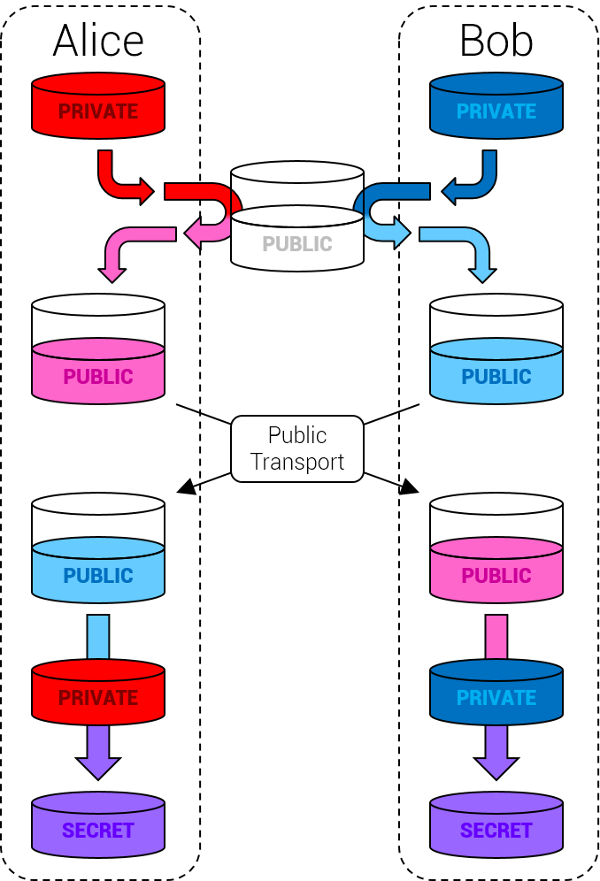
\includegraphics[height=.85\textheight]{diffie-hellman-paint.png}
      \fontsize{8pt}{8pt}\selectfont
      Imagem obtida em
      \url{http://crypto.mdc.io/2012/10/13/public-key-cryptography/}
    \end{center}
    \column{.6\textwidth}
    \resizebox{\textwidth}{!}{%
      \begin{tabular}{rl}
        Número primo (público): & $p$ \\
        Base (público): & $g$ \\
        Chave privada da Alice: & $a$ \\
        Chave pública da Alice: & $A = g^a \mod p$ \\
        Chave privada do Bob: & $b$ \\
        Chave pública do Bob: & $B = g^b \mod p$ \\
        Número compartilhado: & $A^b \equiv B^a \mod p$
      \end{tabular}%
    }
    \vfill
    \vspace{-.5em}
    \begin{minted}{python}
      # Alice e Bob combinam os parâmetros
        p = 2551  ;  g = 2        # Python
      # Criam chaves privadas em silêncio
        a = 47    ;  b = 29
      # Calculam e trocam chaves públicas
        A = (g ** a) % p          # 2285
        B = (g ** b) % p          # 207
      # Alice e Bob possuem um segredo!
        secret_b = (A ** b) % p   # 414
        secret_a = (B ** a) % p   # 414
    \end{minted}
    \begin{center}
      \vspace{-1.5em}
      Se tivéssemos \challengeFour, qual seria o segredo?
    \end{center}
  \end{columns}
\end{frame}


\begin{frame}[fragile]{GPG: \texttt{-c}/\texttt{--symmetric},
                            \texttt{-o}/\texttt{--output} e
                            \texttt{-d}/\texttt{--decrypt}}
  O GPG (\emph{GNU Privacy Guard})
  é uma implementação em software livre (GPLv3)
  que atende ao OpenPGP\footnote{
      PGP significa \emph{Pretty Good Privacy},
      um software comercial criado em 1991.
      Sua segunda versão formou o [hoje obsoleto] padrão RFC1991.
      A menos de uma atualização relativa ao algoritmo Camellia,
      RFC4880 (OpenPGP) é a versão mais recente do padrão.
    }
  sem utilizar softwares/algoritmos patenteados/restritos/privados.
  \vfill
  Exemplo de uso para criptografia de chave simétrica:
  \vfill
  \begin{minted}{shell}
    echo 'Tô na EACH!' > m.txt # Armazena uma a mensagem
    gpg -c -o m.txt.gpg m.txt  # Encriptação! GPG pede senha 2x
    hexdump -C m.txt.gpg       # O resultado é binário...
    file m.txt.gpg             # ... com metadados abertos
    killall gpg-agent          # Para o GPG "esquecer a senha"
    gpg -d m.txt.gpg > m_decrypted.txt     # Decriptação!
  \end{minted}
\end{frame}


\begin{frame}[fragile]{GPG: \texttt{-b}/\texttt{--detach-sign},
                            \texttt{--verify} e
                            \texttt{-e}/\texttt{--encrypt}}
  \vspace{-1em}
  \begin{minted}{shell}
    gpg --gen-key # Criar chaves (par público/privado)
    gpg -k        # Lista keyIDs disponíveis

    # Exportando/importando chaves públicas (para um dado keyID)
    gpg --keyserver pgp.mit.edu --send-keys keyID  # Envio
    gpg --keyserver pgp.mit.edu --recv-keys keyID  # Recebimento
    gpg --export --armor danilo.bellini@gmail.com > my.key
    gpg --import my.key

    # Assinatura em arquivo à parte (--detach-sign)
    gpg -u email@example.br -b m.txt  # Assina (cria m.txt.sig)
    gpg --verify m.txt.sig m.txt      # Verifica a assinatura

    # Encriptando (--encrypt) c/ a chave pública do destinatário
    gpg -o encrypted.gpg -r destino@example.br -e m.txt

    # Decriptando (--decrypt) com a chave privada
    gpg -o decrypted.txt -d encrypted.gpg
  \end{minted}
  \vfill
  \vspace{-.5em}
  O \mintinline{shell}{-u/--local-user}
  define a chave privada que assina,
  o \mintinline{shell}{-r/--recipient} define o destinatário.
  O \mintinline{shell}{-R/--hidden-recipient}
  não armazena o keyID do destinatário no resultado.
\end{frame}


\begin{frame}[fragile]{Tomb: armazenamento criptografado em um arquivo}
  Discos rígidos, SSDs, SDs, etc.
  normalmente não estão criptografados,
  mas o \emph{Tomb} permite criar arquivos
  que funcionam como ``diretórios criptografados''.
  \vfill
  \begin{minted}{shell}
    tomb dig new.tomb -s 50  # Cria o new.tomb com 50MB
    # A criptografia a ser aplicada no new.tomb é feita
    # por meio de uma chave (simétrica) gerada pelo Tomb,
    # a qual será encriptada com o GPG por meio de ...

    # Senha (chave simétrica), ou ...
    tomb forge new.key
    tomb lock new.tomb -k new.key  # Inicializa e formata
    tomb open new.tomb -k new.key  # Monta
    tomb close new                 # Desmonta

    # Chave pública (via GPG)
    tomb forge new.key -g -r email@example.br
    tomb lock new.tomb -k new.key -g -r email@example.br
    # Dica: depois do -k são os mesmos parâmetros do forge
  \end{minted}
\end{frame}


\begin{frame}[fragile]{Esteganografia}
  \textbf{Esteganografia}: ocultação de uma informação dentro de outra.
  Ocultaremos em uma imagem a chave usada
  para acesso ao Tomb (via Steghide\footnote{
    \url{http://steghide.sourceforge.net/}
  }).
  \vfill
  \begin{minted}{shell}
    # Cria uma cópia de um JPG (pode ser uma foto)
    cp IXSSI-768x294.jpg fakelogo.jpg

    # Armazena a chave na imagem, usando uma senha
    tomb bury fakelogo.jpg -k new.key

    # Para extrair a chave da imagem (sabendo a senha)
    tomb exhume fakelogo.jpg -k copy.key

    # Podemos usar a própria imagem como arquivo de chave
    tomb open new.tomb -k fakelogo.jpg
  \end{minted}
  \vfill
  Não deverá haver diferença visual perceptível,
  e somente o portador da senha sabe que há uma chave nessa imagem.
\end{frame}


\begin{frame}{\emph{Hash} e criptografia ``sem chave''}
  Exemplos de algoritmos:
  \begin{itemize}
    \item \emph{Checksum} e dígitos verificadores
          (CPF, CNPJ, RG, ISSN, etc.)
    \item MD5
    \item SHA-1 (torrents, git)
    \item SHA-2 (SHA-224, SHA-256, SHA-384, SHA-512,
                 SHA-512/224, SHA-512/256)
  \end{itemize}
  \vspace{.5em}
  \vfill
  Exemplo DV \textbf{Módulo 11} (ISSN):
  \emph{Psicologia USP} (0103-6564)
  \[
  \begin{array}{rccccccccl}
    \text{ISSN:} &  0 &  1 &  0 &  3 & - &  6 &  5 &  6 & (4) \\
          \times &  8 &  7 &  6 &  5 &   &  4 &  3 &  2 \\ \hline
      S = \sum & \{ 0,&  7,&  0,& 15,&   & 24,& 15,& 12 \} & = 73 \\
  \end{array}
  \]
  O resto da divisão por $11$ é $7$, e o complemento é $11 - 7 = 4$,
  o dígito verificador.
  \[
  73 = 11 \cdot 6 + {\underset{\uparrow}{7}} =
       11 \cdot 7 - {\underset{\uparrow}{4}}
  \]
  \begin{center}\Large
    Qual o dígito verificador do ISSN \texttt{\challengeFive}?
  \end{center}
\end{frame}


\begin{frame}[fragile]{\emph{Hash},
              funções de espalhamento ou dispersão criptográfica}
  Valor, código \emph{hash}, \emph{digest}, ou resumo:
  resultado de uma função de \emph{hash} p/ uma mensagem.
  Para criptografia, tais funções devem ser:
  \begin{itemize}
    \item Determinísticas
          (mesma mensagem $\Rightarrow$ mesmo \emph{hash})
    \item ``Caóticas'' (pequenas mudanças na mensagem de entrada
                        mudam o \emph{hash} completamente)
    \item Extremamente difíceis de reverter
          (somente podemos obter a mensagem a partir do \emph{hash}
           por tentativa e erro)
    \item Extremamente difíceis de colidir
          (idealmente nunca encontramos
           mensagens diferentes com o mesmo \emph{hash})
  \end{itemize}
  \vspace{.5em}
  \vfill
  Exemplo em \emph{Python}:
  \vspace{-.5em}
  \begin{minted}{python}
    >>> import hashlib                  # Biblioteca padrão
    >>> with open("m.txt", "rb") as msg_file:
    ...     msg = msg_file.read()

    >>> # Tem sha224, md5, sha256, sha1, ...
    >>> hashlib.sha224(msg).hexdigest()
    '818bd235f6995df200dea5dc77c9d01be4a5ad8d8447b0a3b3dcc107'
  \end{minted}
\end{frame}


\begin{frame}
  \begin{columns}[c]
    \column{.68\textwidth}
    Há muito mais sobre o assunto! Exemplos:
    \begin{itemize}
      \item Algoritmo de Shamir (particionar chave)
      \item TLS/SSL (e.g. HTTPS)
      \item Quando e por que usar criptografia?
      \item TOTP, HMAC, gerenciamento de senhas
      \item Como funciona a validação dos certificados
            da Python Sudeste 2018?
    \end{itemize}
    \vspace{-.8em}
    \begin{center}
      \qrcode[height=5cm]{\repo}
    \end{center}
    \column{.48\textwidth}
    {\hfill \textbf{Desafios}}
    \begin{itemize}
      \item \emph{Cifra de César} \\
        \texttt{\challengeOne}
        (Chave: \texttt{\challengeOneKey})
      \item \emph{Cifra de Vigenère} \\
        \texttt{\challengeTwo}
        (Chave: \texttt{\challengeTwoKey})
      \item \emph{Auto-chave} \\
        \texttt{\challengeThree}
        (Chave: \texttt{\challengeThreeKey})
      \item \emph{Diffie-Hellman}:
        \challengeFour
      \item \emph{Dígito ISSN}
        \texttt{\challengeFive}
    \end{itemize}
    \vfill
    \begin{center}
      {\fontsize{5cm}{2.5cm}\selectfont FIM!}
      \vfill
      \vspace{.5em}
      \url{\repo}
    \end{center}
  \end{columns}
\end{frame}


\end{document}
